\documentclass[14pt]{beamer}
\usepackage{./Estilos/BeamerUVM}
\usepackage{./Estilos/ColoresLatex}
\usetheme{Madrid}
\usecolortheme{default}
%\useoutertheme{default}
\setbeamercovered{invisible}
% or whatever (possibly just delete it)
\setbeamertemplate{section in toc}[sections numbered]
\setbeamertemplate{subsection in toc}[subsections numbered]
\setbeamertemplate{subsection in toc}{\leavevmode\leftskip=3.2em\rlap{\hskip-2em\inserttocsectionnumber.\inserttocsubsectionnumber}\inserttocsubsection\par}
% \setbeamercolor{section in toc}{fg=blue}
% \setbeamercolor{subsection in toc}{fg=blue}
% \setbeamercolor{frametitle}{fg=blue}
\setbeamertemplate{caption}[numbered]

\setbeamertemplate{footline}
\beamertemplatenavigationsymbolsempty
\setbeamertemplate{headline}{}


\makeatletter
% \setbeamercolor{section in foot}{bg=gray!30, fg=black!90!orange}
% \setbeamercolor{subsection in foot}{bg=blue!30}
% \setbeamercolor{date in foot}{bg=black}
\setbeamertemplate{footline}
{
  \leavevmode%
  \hbox{%
  \begin{beamercolorbox}[wd=.333333\paperwidth,ht=2.25ex,dp=1ex,center]{section in foot}%
    \usebeamerfont{section in foot} {\insertsection}
  \end{beamercolorbox}%
  \begin{beamercolorbox}[wd=.333333\paperwidth,ht=2.25ex,dp=1ex,center]{subsection in foot}%
    \usebeamerfont{subsection in foot}  \insertsubsection
  \end{beamercolorbox}%
  \begin{beamercolorbox}[wd=.333333\paperwidth,ht=2.25ex,dp=1ex,right]{date in head/foot}%
    \usebeamerfont{date in head/foot} \insertshortdate{} \hspace*{2em}
    \insertframenumber{} / \inserttotalframenumber \hspace*{2ex} 
  \end{beamercolorbox}}%
  \vskip0pt%
}
\makeatother

\makeatletter
\patchcmd{\beamer@sectionintoc}{\vskip1.5em}{\vskip0.8em}{}{}
\makeatother

% \usefonttheme{serif}
\usepackage[clock]{ifsym}

\sisetup{per-mode=symbol}
\resetcounteronoverlays{saveenumi}

\title{\Large{Práctica 1 - Ondas mecánicas} \\ \normalsize{Física IV (Área II)}}
\date{}

\renewcommand\cellset{\renewcommand\arraystretch{0.7}%
\setlength\extrarowheight{0pt}}

\addtobeamertemplate{frametitle}{}{%
\begin{tikzpicture}[remember picture,overlay]
\coordinate (logo) at ([xshift=-1.5cm,yshift=-0.8cm]current page.north east);
% \fill[devryblue] (logo) circle (.9cm);
% \clip (logo) circle (.75cm);
\node at (logo) {
\includegraphics[width=2.1cm]{Imagenes/logo_UVM.png}};
\end{tikzpicture}}

\begin{document}
\maketitle

\section*{Contenido}
\frame{\frametitle{Contenido} \tableofcontents[currentsection, hideallsubsections]}

\section{Ondas estacionarias}
\frame{\tableofcontents[currentsection, hideothersubsections]}
\subsection{El concepto}

\begin{frame}
\frametitle{La onda estacionaria}
Las \textocolor{carmine}{ondas estacionarias} no son ondas de propagación sino los distintos \textocolor{blue-violet}{modos de vibración} de una cuerda, una membrana, etc.
\end{frame}
\begin{frame}
\frametitle{La onda estacionaria}
Cuando dos trenes de onda de la misma frecuencia, velocidad y amplitud, \pause viajan en sentidos opuestos, la \textocolor{coquelicot}{superposición} de ellos da lugar a ondas estacionarias.
\end{frame}
\begin{frame}
\frametitle{La onda estacionaria}
Una de las características más importantes de estas ondas es el hecho de que la \textocolor{cobalt}{amplitud de la oscilación} no es la misma para diferentes puntos, \pause sino que \textocolor{lava}{varía con la posición} de ellos.
\end{frame}
\begin{frame}
\frametitle{El nodo de la onda}
Hay puntos que no oscilan, es decir, tienen \textocolor{cadetblue}{amplitud cero}; \pause dichas posiciones se llaman \textocolor{ao}{nodos}.
\end{frame}
\begin{frame}
\frametitle{El antinodo de la onda}
También hay puntos que oscilan con \textocolor{byzantium}{amplitud máxima}; esas posiciones se llaman \textocolor{red}{antinodos}.
\end{frame}
\begin{frame}
\frametitle{Nodos y antinodos}
\begin{figure}
    \centering
    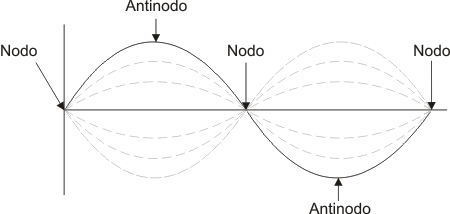
\includegraphics[scale=0.6]{Imagenes/Onda_Estacionaria_01.png}
\end{figure}
\end{frame}
\begin{frame}
\frametitle{Generando ondas estacionarias}
En una cuerda fija en ambos extremos, se pueden formar ondas estacionarias de modo que siempre los puntos extremos son nodos. 
\end{frame}
\begin{frame}
\frametitle{Generando ondas estacionarias}
La cuerda puede oscilar con distintas formas denominadas modos de vibración, con nodos entre sus extremos, \pause de tal manera que las longitudes de onda correspondientes a las ondas estacionarias cumplen con la relación:
\pause
\begin{align}
n \dfrac{\lambda}{2} = L
\label{eq:ecuacion_01}
\end{align}
\end{frame}
\begin{frame}
\frametitle{La expresión de la onda}
\begin{align*}
n \dfrac{\lambda}{2} = L
\end{align*}
donde $L$ es el largo de la cuerda y $n$ son los armónicos.
\end{frame}
\begin{frame}
\frametitle{Los armónicos n = 1}
\begin{figure}
    \centering
    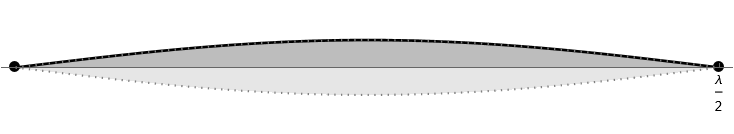
\includegraphics[width=\linewidth]{Imagenes/Practica_01_01.png}
\end{figure}
\end{frame}
\begin{frame}
\frametitle{Los armónicos n = 2}
\begin{figure}
    \centering
    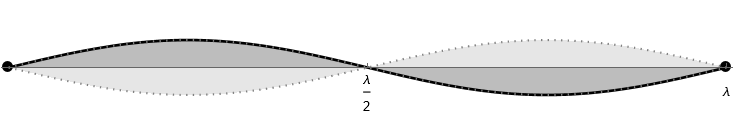
\includegraphics[width=\linewidth]{Imagenes/Practica_01_02.png}
\end{figure}
\end{frame}
\begin{frame}
\frametitle{Los armónicos n = 3}
\begin{figure}
    \centering
    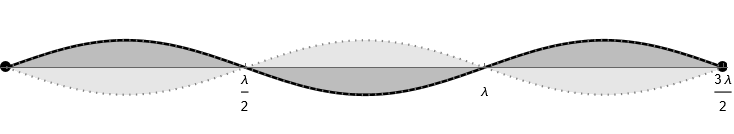
\includegraphics[width=\linewidth]{Imagenes/Practica_01_03.png}
\end{figure}
\end{frame}
\begin{frame}
\frametitle{Los armónicos n = 4}
\begin{figure}
    \centering
    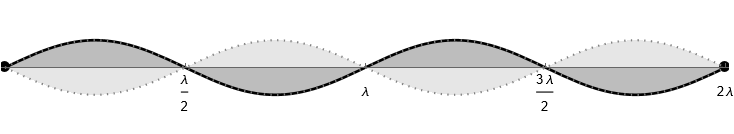
\includegraphics[width=\linewidth]{Imagenes/Practica_01_04.png}
\end{figure}
\end{frame}
\end{document}